\section{Sensorik}

\begin{frame}{Sensorik}{Anforderungen}
  \begin{itemize}
    \item Welche Daten brauchen wir?
    \begin{itemize}
    \item Kommutierungszeitpunkt
    \item Umdrehungsgeschwindigkeit
    \item Drehwinkel
    \item Temperatur
    \end{itemize}
    \item Welche Sensoren stehen zur Verfügung?
    \begin{itemize}
      \item Drei Hall-Sensoren
      \item Inkrementalgeber
      \item NTC Temperatursensor
    \end{itemize}
  \end{itemize}
\end{frame}

\begin{frame}{Sensorik}{Sensor Interface}	
  \begin{itemize}
    \item Kapselung in ein eigenes Softwaremodul
    \item Zugriff auf Sensorwerte über ein definiertes Interface
    \begin{itemize}
      \item Geringer Integrationsaufwand
      \item Gute Portierbarkeit
    \end{itemize}
  \end{itemize}
  \dirtree{%
  .1 Sensor.h.
  .2 Sensor\_Hall.h.
  .2 Sensor\_QuadratureDecoder.h.
  .2 Sensor\_Temperature.h.
  }  
\end{frame}

\begin{frame}{Sensorik}{Sensor Interface}	
 \begin{figure} [htbp]
  \centering
  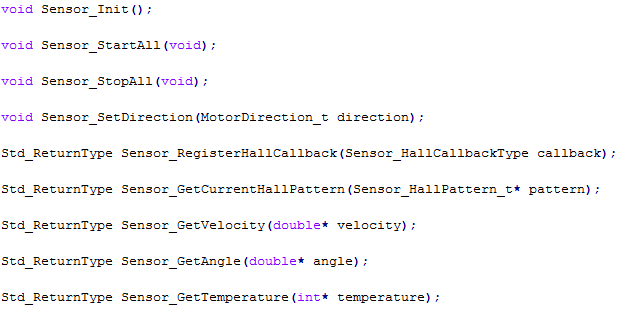
\includegraphics[scale=0.6]{Sensor/sensor_interface.PNG}
 \end{figure}
\end{frame}

\begin{frame}{Sensorik}{Hall-Sensoren}	
 Digitale Hall-Sensoren zur Messung von Magnetfeldern
 \begin{figure} [htbp]
  \centering
  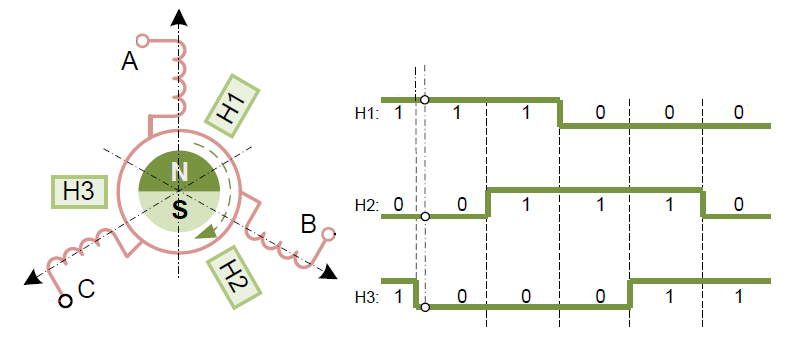
\includegraphics[scale=0.4]{Sensor/hall_sample.PNG}
 \end{figure}
\end{frame}

\begin{frame}{Sensorik}{Hall-Sensoren}	
 \begin{itemize}
 \item Messung des Hall-Patterns mit POSIF
 \item Zwei mögliche Events
	 \begin{itemize}
	 \item Correct-Hall-Event
	 \item Wrong-Hall-Event
	 \end{itemize}
 \item Ermittlung des motorspezifischen Hall-Patterns
 \end{itemize}
 \begin{figure} [htbp]
   \centering
   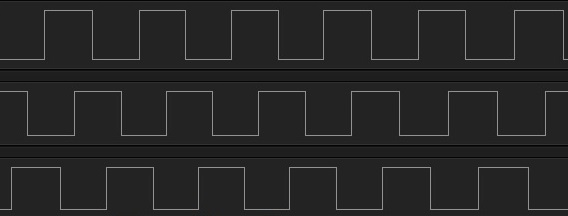
\includegraphics[scale=0.3]{Sensor/hall_pattern.jpg}
  \end{figure}
\end{frame}

\begin{frame}{Sensorik}{Inkrementalgeber}	
 \begin{itemize}
 \item Messung Umdrehungsgeschwindigkeit
 \item Messung Drehwinkel der Welle
 \item Drei Signalleitungen
 \begin{itemize}
 \item Indexleitung
 \item Phase A
 \item Phase B
 \end{itemize}
 \end{itemize}
 \begin{figure} [htbp]
   \centering
   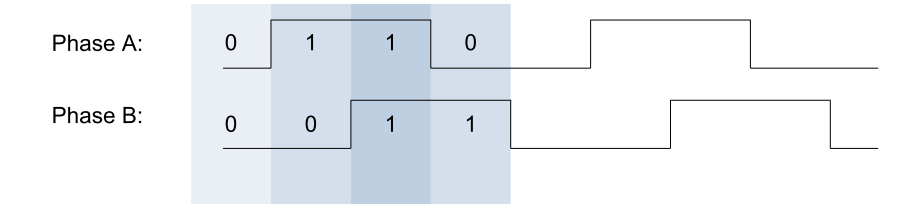
\includegraphics[scale=0.4]{Sensor/quadrature_overview.PNG}
 \end{figure}
\end{frame}

\begin{frame}{Sensorik}{Inkrementalgeber}	
 \begin{itemize}
 \item Mögliche Implementierungsstrategien
 \begin{itemize}
 \item POSIF + CCU
 \item Zwei CCU Slices
 \end{itemize}
 \end{itemize}
\end{frame}

\begin{frame}{Sensorik}{Temperatursensor}	
 \begin{itemize}
 \item NTC Widerstand
 \begin{itemize}
 \item Sinkender Widerstand bei steigender Temperatur
 \end{itemize}
 \item Temperaturermittlung durch Datenblatt
 \item Widerstand nicht direkt messbar
 \begin{itemize}
 \item Messung durch Spannungsteiler
 \end{itemize}
 \end{itemize}
 \begin{figure} [htbp]
 \centering
 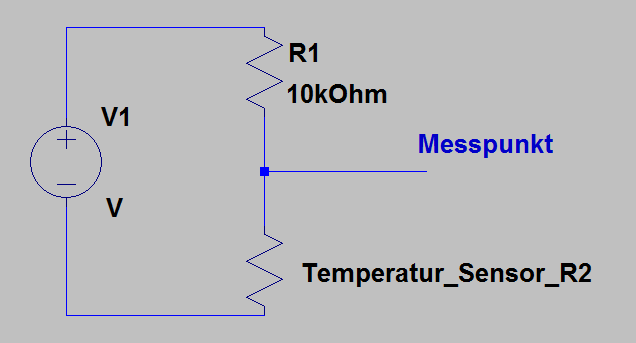
\includegraphics[scale=0.3]{Sensor/temperature_circuit.PNG}
 \end{figure}
\end{frame}

\begin{frame}{Sensorik}{Temperatursensor}	
Berechnung des Widerstands
\begin{equation}
U_{2} = \frac{U_{ges}}{R_{1} + R_{2}} * R_{2}
\end{equation}
Umstellen auf R2 durch Äquivalenzumformung
\begin{equation}
R_{2} = \frac{U_{2} * R_{1}}{U_{ges} - U_{2}}
\end{equation} 
\end{frame}

\begin{frame}{Sensorik}{Ausblick}	
 \begin{itemize}
 \item Portierung auf anderen Controller
 \item Nutzung des Inkrementalsgebers als Basis für die Kommutierung
 \end{itemize}
\end{frame}